\documentclass[runningheads]{llncs}

\usepackage[utf8]{inputenc}
\usepackage[T1]{fontenc}
\usepackage[english]{babel}
\usepackage{amsmath,amssymb}
\usepackage{graphicx}
\graphicspath{{figures/}}
\usepackage{multirow}
\usepackage{array}
\usepackage{hyperref}
\usepackage{algorithm}
\usepackage{algorithmic}
\usepackage{url}
\usepackage{microtype}
\usepackage{xcolor}
\usepackage{tikz}
\usetikzlibrary{arrows.meta,positioning,shapes.geometric,calc,fit,backgrounds}
\definecolor{modblue}{RGB}{200,220,240}
\definecolor{modgreen}{RGB}{200,235,200}
\definecolor{modorange}{RGB}{255,225,180}
\definecolor{modred}{RGB}{245,200,200}
\definecolor{modgray}{RGB}{235,235,235}
\definecolor{decyellow}{RGB}{255,245,180}

\renewcommand\UrlFont{\rmfamily}

\begin{document}

\title{GNN-ReGVD+: A Vulnerability Detection Pipeline for C/C++ Code with Execution-Based Verification}

\titlerunning{GNN-ReGVD+: Vulnerability Detection Pipeline}

\author{A.\,V.~Antonov\inst{1} \and
V.\,S.~Burovin\inst{1} \and
V.\,S.~Voevodkin\inst{1}}

\authorrunning{A.\,V. Antonov et al.}

\institute{HSE University, Nizhny Novgorod campus, Nizhny Novgorod, Russia\\
\email{\{avantonov,vsburovin\}@edu.hse.ru, b.voevodkin@gmail.com}}

\maketitle

% ====================================================================
%                        ABSTRACT
% ====================================================================
\begin{abstract}
Automatic vulnerability detection in C/C++ source code using graph neural networks is characterized by a significant level of false positives in the absence of execution-based exploitability confirmation. This paper proposes the GNN-ReGVD+ pipeline, which integrates four modules: (1)~neural network detection based on the ReGVD model with parameter-efficient LoRA adaptation and hybrid scoring via FAISS; (2)~retrieval of relevant exploit templates from a vector database; (3)~cascading template adaptation using large language models; (4)~execution-based verification in a Docker-isolated environment with multi-sanitizer support and coverage-guided fuzzing. Experimental evaluation on the Devign (27,318 functions) and MegaVul (339,548 functions) datasets demonstrated that the hybrid architecture does not degrade the baseline model performance ($\Delta < 0.5$~p.p.), LoRA adaptation of 0.12\% of parameters yields a ROC-AUC improvement of $+0.179$ during domain transfer with a 1.8$\times$ reduction in VRAM consumption, and the sandbox verification module covers 18 vulnerability types (23~CWEs) with a four-level evidence classification. The system is implemented as 9,372 lines of Python code with 203 automated tests.

\keywords{vulnerability detection \and graph neural networks \and LoRA \and FAISS \and sandbox verification \and fuzzing \and DevSecOps}
\end{abstract}

% ====================================================================
%                     1. INTRODUCTION
% ====================================================================
\section{Introduction}

The growing volume of software and the increasing frequency of cyberattacks intensify the need for automated vulnerability detection tools for source code~\cite{nist800}. According to OWASP~\cite{owasp2024}, code-level vulnerabilities remain one of the leading attack vectors against web applications and system infrastructure, with the number of published CVEs increasing annually. Traditional static analysis (SAST) tools, such as SonarQube, CodeQL, Coverity, and Semgrep, provide interpretable and reproducible results; however, they are characterized by high false positive rates---from 30 to 80\%~\cite{sultana2024}---and dependence on manually crafted rules. Each rule requires expert knowledge of a specific vulnerability class, making tool scalability labor-intensive and error-prone.

Deep learning methods represent an alternative approach to this task. Graph neural networks (GNNs)~\cite{nguyen2022regvd,zhou2019devign} model structural dependencies in program code, while pretrained code models (GraphCodeBERT~\cite{guo2021graphcodebert}, CodeLlama, DeepSeek-Coder) capture semantic patterns from large corpora~\cite{ding2024}. These approaches improve detection accuracy compared to manual rules; however, they share a fundamental limitation: all of them produce only a binary classification of a code fragment (vulnerable / not vulnerable) without providing execution-based evidence of exploitability. Without such evidence, developers must manually analyze each warning, which reduces trust in automated tools and slows down the remediation process~\cite{gajjar2026vbf}. As a consequence, a significant portion of warnings is ignored, and real vulnerabilities may be missed among the flood of false positives.

This work aims to overcome this limitation. We propose the GNN-ReGVD+ pipeline, in which neural network detection is augmented with automatic proof-of-concept exploit generation and their verification in an isolated environment. The pipeline is designed as a funnel: lightweight GNN detection quickly filters out safe code, while resource-intensive operations (LLM-based exploit adaptation, Docker verification) are applied only to suspicious fragments. This architecture ensures a balance between analysis speed and verification depth.

The main contributions of this work are:

\begin{enumerate}
    \item An integrated four-module architecture combining GNN detection with hybrid scoring, FAISS-based exploit template retrieval, cascading LLM adaptation, and sandbox verification with a parallel LLM triage branch.
    \item A hybrid scoring method ReGVD+FAISS with LoRA adaptation (0.12\% of parameters), achieving a ROC-AUC improvement of $+0.179$ during domain transfer with a 1.8$\times$ VRAM reduction.
    \item Multi-sanitizer execution-based verification covering 18~vulnerability types through three profiles (ASan+UBSan, MSan, TSan), coverage-guided fuzzing, and four-level evidence classification with automatic CWE mapping (23~entries).
    \item A reproducible implementation---9,372 lines of Python code, 203~automated tests, and a CLI interface for CI/CD integration.
\end{enumerate}

The paper is organized as follows. Section~2 reviews existing approaches to vulnerability detection and related work. Section~3 describes the architecture of the GNN-ReGVD+ pipeline. Section~4 presents the implementation and testing details. Section~5 provides the experimental evaluation results. Section~6 discusses the findings and limitations. Section~7 contains the conclusion.


% ====================================================================
%                  2. RELATED WORK
% ====================================================================
\section{Related Work}

The task of automated vulnerability detection in source code has a long research history. In this section, we review the evolution of approaches from static analysis to modern deep learning methods and formulate the research gap that motivates this work.

\textbf{Static analysis and classical machine learning.}
Early approaches to automated vulnerability detection relied on manually written rules and patterns. SAST tools (SonarQube, Coverity, CodeQL, Semgrep) apply fixed rules to the abstract syntax tree or data flow of a program. Despite their high interpretability, they are limited to the vulnerability classes for which rules have been written and generate a significant number of false positives~\cite{sultana2024}. Classical machine learning methods (Random~Forest, SVM, logistic regression) based on engineered features achieved only ROC-AUC in the range of 0.46--0.50, failing to capture semantic patterns of vulnerable code. The transition to deep learning on sequences (LSTM, TextCNN, Transformer) eliminated the need for manual feature engineering; however, linear token processing did not capture structural program dependencies---control flow, data dependencies, call nesting.

\textbf{Graph neural networks.}
Graph neural networks (GNNs) emerged as a response to this limitation, representing a program as a graph where nodes correspond to code elements and edges represent structural and semantic relationships between them. The Devign model~\cite{zhou2019devign} demonstrated the effectiveness of this approach by combining control flow graph (CFG) and program dependence graph (PDG) representations with gated GNN layers. ReGVD~\cite{nguyen2022regvd} simplified the approach by proposing graph construction directly from code tokens via a fixed-size sliding window mechanism, eliminating the need for a separate parsing stage. The model uses residual connections to stabilize the training of deep graph networks and soft attention pooling to aggregate node representations, achieving F1~$\approx 0.72$ on the Devign dataset.

Specialized detection work, particularly use-after-free vulnerability detection via deep graph learning~\cite{chen2024uaf}, has shown the promise of GNNs for specific defect classes. However, a systematic study by Ding et al.~\cite{ding2024} revealed that under proper experimental design (deduplication, data distribution control), the reported metrics of many models decrease significantly, pointing to reproducibility issues in the field. Despite this, GNNs remain one of the most promising directions due to their ability to model structural properties of programs.

\textbf{Pretrained code language models.}
Pretrained models (GraphCodeBERT~\cite{guo2021graphcodebert}, CodeLlama, DeepSeek-Coder, StarCoder) achieve ROC-AUC of 80--83\% in zero-shot mode~\cite{ding2024}, making them attractive for vulnerability detection without training on specialized data. SAST-Genius~\cite{agrawal2025sast} applies large language models (LLMs) for triaging CodeQL static analysis alerts by extracting graph context to improve classification accuracy. The neuro-symbolic approach by Li et al.~\cite{li2025neurosymbolic} combines LLM vulnerability patterns with static analysis. Comparative studies~\cite{sultana2024,makhyari2024} confirmed that LLMs detect semantically complex patterns but suffer from inference instability and high computational cost. All reviewed approaches are limited to binary code classification without exploitability confirmation.

\textbf{Execution-based verification and fuzzing.}
The Verify Before You Fix concept~\cite{gajjar2026vbf} formalizes the idea of execution-based validation through a Docker sandbox with evidence classification (CONFIRMED / SUGGESTIVE / INCONCLUSIVE). This approach proposes first confirming the presence of a vulnerability by running exploit code in an isolated environment and only then proceeding with remediation. Fuzzing has evolved from random input mutation (AFL) to coverage-guided approaches (LibFuzzer, Honggfuzz), which use code coverage information to guide test generation. Memory sanitizers (ASan, MSan, TSan) complement fuzzing by detecting errors that do not cause immediate crashes but represent serious vulnerabilities---reads of uninitialized memory, data races, and out-of-bounds accesses without SIGSEGV.

\textbf{Parameter-efficient adaptation.}
LoRA (Low-Rank Adaptation)~\cite{hu2021lora} adds compact trainable low-rank matrices ($r \ll \min(d, k)$) to the attention layers of a pretrained model while keeping the remaining parameters frozen. Unlike full fine-tuning, LoRA requires storing and updating only a small fraction of parameters, significantly reducing computational resource requirements. In the context of vulnerability detection, LoRA is promising for domain transfer: a model trained on one dataset can be adapted to a new codebase with a different vulnerability distribution without full retraining.

\textbf{Research gap.}
A comparison of existing paradigms (Table~\ref{tab:paradigms}) reveals the key gap: none of the reviewed approaches combines fast GNN detection with execution-based verification. Classical ML is limited in accuracy, GNNs provide a good balance of speed and quality, and LLMs offer the best accuracy but at high computational cost. Yet, all three paradigms terminate at the classification stage without providing exploitability evidence. GNN-ReGVD+ fills this gap by implementing a complete cycle from detection to sandbox verification with automatic CWE mapping.

\begin{table}
\centering
\caption{Comparison of automated vulnerability analysis paradigms}
\label{tab:paradigms}
\small
\begin{tabular}{|p{2.0cm}|p{2.6cm}|p{2.8cm}|p{3.0cm}|}
\hline
\textbf{Criterion} & \textbf{Classical ML} & \textbf{GNN (ReGVD)} & \textbf{LLM (CodeLlama)} \\
\hline
Representation & Engineered features & Graphs (sliding window) & Token sequences \\
Accuracy & ROC-AUC $\approx$ 0.46--0.50 & Acc $\approx$ 62--64\% & ROC-AUC 80--83\% \\
Latency & Microseconds & Milliseconds & Seconds \\
Adaptability & Low & Medium (LoRA) & High (zero-shot) \\
Verification & No & No & No \\
\hline
\end{tabular}
\end{table}


% ====================================================================
%              3. PIPELINE ARCHITECTURE
% ====================================================================
\section{Architecture of the GNN-ReGVD+ Pipeline}

This section describes the architecture of the proposed pipeline. The system consists of four sequential modules: GNN detection with hybrid scoring, exploit template retrieval from a vector database, cascading LLM-based template adaptation, and sandbox verification in a Docker-isolated environment. In parallel with the main pipeline, an LLM triage head operates, providing an independent semantic analysis channel. The overall architecture is shown in Fig.~\ref{fig:pipeline}.

\begin{figure}
\centering
\resizebox{\textwidth}{!}{%
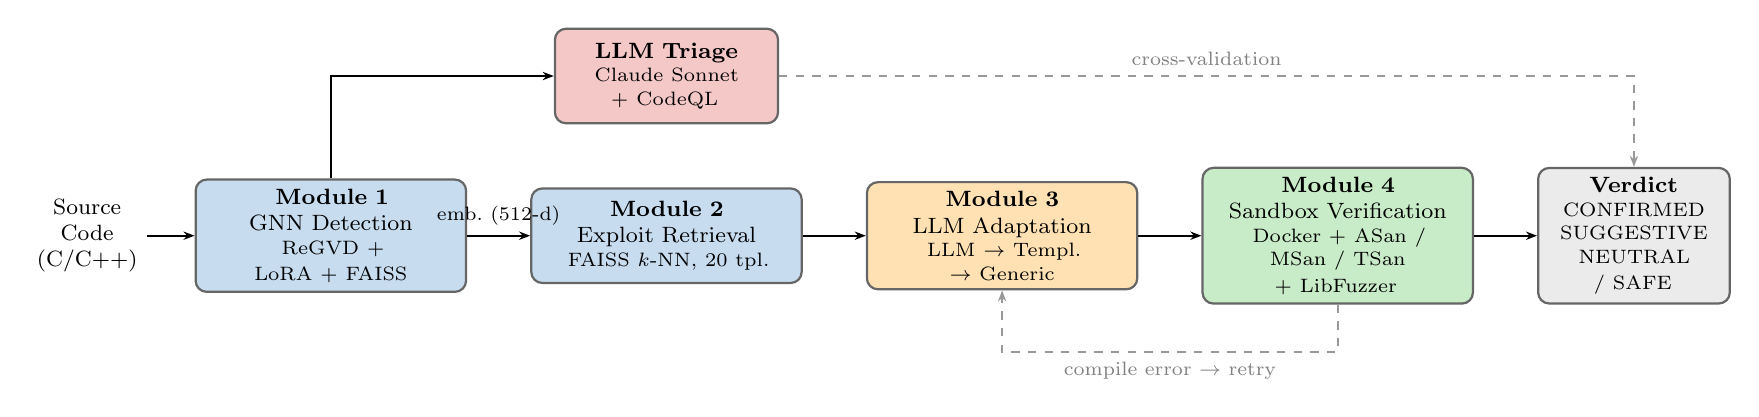
\begin{tikzpicture}[
    module/.style={rectangle, draw=black!60, rounded corners=4pt, minimum height=1.2cm,
        text width=3.2cm, align=center, font=\footnotesize, line width=0.8pt},
    arr/.style={-{Stealth[length=4pt]}, semithick},
    darr/.style={-{Stealth[length=4pt]}, semithick, dashed, draw=black!40},
    node distance=0.8cm
]
\node[module, fill=modblue] (m1) {\textbf{Module 1}\\GNN Detection\\[-1pt]{\scriptsize ReGVD + LoRA + FAISS}};
\node[module, fill=modblue, right=of m1] (m2) {\textbf{Module 2}\\Exploit Retrieval\\[-1pt]{\scriptsize FAISS $k$-NN, 20 tpl.}};
\node[module, fill=modorange, right=of m2] (m3) {\textbf{Module 3}\\LLM Adaptation\\[-1pt]{\scriptsize LLM $\to$ Templ.}\\[-1pt]{\scriptsize $\to$ Generic}};
\node[module, fill=modgreen, right=of m3] (m4) {\textbf{Module 4}\\Sandbox Verification\\[-1pt]{\scriptsize Docker + ASan /}\\[-1pt]{\scriptsize MSan / TSan + LibFuzzer}};

\node[left=0.6cm of m1, font=\footnotesize, align=center] (input) {Source\\Code\\(C/C++)};
\draw[arr] (input) -- (m1);
\draw[arr] (m1) -- node[above, font=\scriptsize] {emb.\ (512-d)} (m2);
\draw[arr] (m2) -- (m3);
\draw[arr] (m3) -- (m4);

\node[rectangle, draw=black!60, rounded corners=4pt, right=0.8cm of m4, align=center,
    font=\footnotesize, minimum height=1.0cm, text width=2.2cm, fill=modgray, line width=0.8pt]
    (verdict) {\textbf{Verdict}\\[-1pt]{\scriptsize CONFIRMED}\\[-1pt]{\scriptsize SUGGESTIVE}\\[-1pt]{\scriptsize NEUTRAL / SAFE}};
\draw[arr] (m4) -- (verdict);

\node[module, fill=modred, text width=2.6cm, above=0.8cm of m2] (triage)
    {\textbf{LLM Triage}\\[-1pt]{\scriptsize Claude Sonnet}\\[-1pt]{\scriptsize + CodeQL}};
\draw[arr] (m1.north) |- (triage.west);
\draw[darr] (triage.east) -| node[near start, above, font=\scriptsize, text=black!50]
    {cross-validation} (verdict.north);

\draw[darr] (m4.south) -- ++(0,-0.6) -| node[near start, below, font=\scriptsize,
    text=black!50] {compile error $\to$ retry} (m3.south);
\end{tikzpicture}%
}
\caption{Architecture of the GNN-ReGVD+ pipeline. Source code passes sequentially through four modules. The LLM triage head operates in parallel. The dashed arrow indicates iterative refinement upon harness compilation failure}
\label{fig:pipeline}
\end{figure}

\subsection{Detection Module: ReGVD with LoRA Adaptation and Hybrid Scoring}

The detection module is based on the ReGVD model~\cite{nguyen2022regvd}, extended with two key components: LoRA adapters for parameter-efficient domain transfer and a FAISS head for hybrid scoring with vulnerability type identification (Fig.~\ref{fig:model}).

\begin{figure}
\centering
\scalebox{0.82}{%
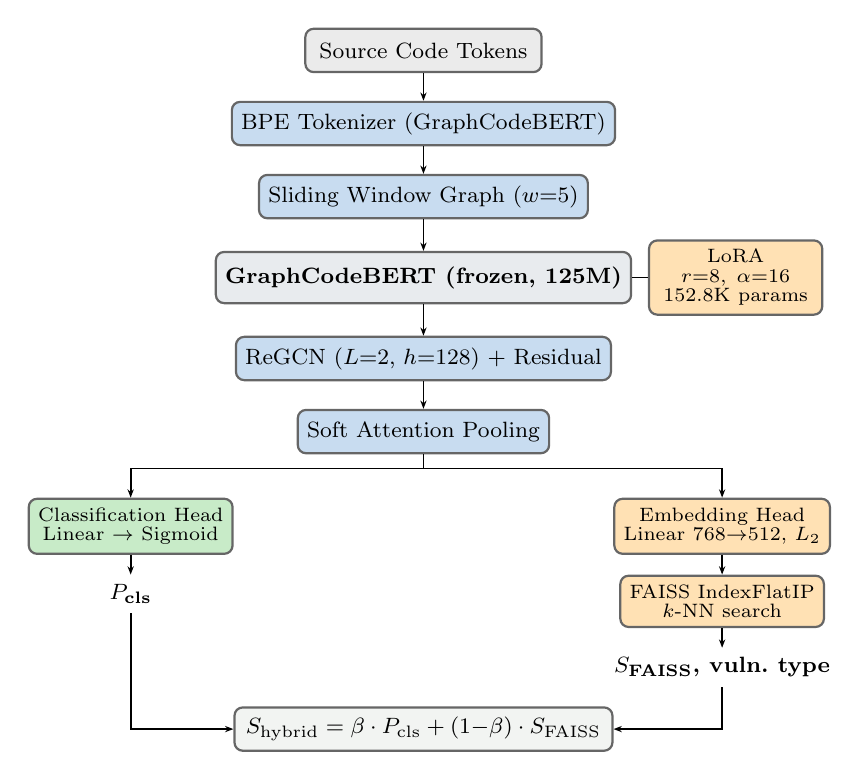
\begin{tikzpicture}[
    block/.style={rectangle, draw=black!60, rounded corners=3pt, minimum width=3.0cm,
        minimum height=0.55cm, align=center, font=\footnotesize, line width=0.8pt},
    sblock/.style={rectangle, draw=black!60, rounded corners=3pt, minimum width=2.2cm,
        minimum height=0.5cm, align=center, font=\scriptsize, line width=0.8pt},
    arr/.style={-{Stealth[length=3pt]}, semithick},
    node distance=0.35cm
]
\node[block, fill=modgray] (input) {Source Code Tokens};
\node[block, fill=modblue, below=of input] (tok) {BPE Tokenizer (GraphCodeBERT)};
\draw[arr] (input) -- (tok);
\node[block, fill=modblue, below=of tok] (graph) {Sliding Window Graph ($w{=}5$)};
\draw[arr] (tok) -- (graph);
\node[block, fill=modblue!70!black!20, below=0.4cm of graph, minimum width=3.6cm,
    minimum height=0.65cm, font=\footnotesize\bfseries] (gcb) {GraphCodeBERT (frozen, 125M)};
\draw[arr] (graph) -- (gcb);
\node[sblock, fill=modorange, right=0.2cm of gcb] (lora) {LoRA\\[-1pt]$r{=}8,\;\alpha{=}16$\\[-1pt]152.8K params};
\draw[semithick] (gcb.east) -- (lora.west);
\node[block, fill=modblue, below=0.4cm of gcb] (regcn) {ReGCN ($L{=}2$, $h{=}128$) + Residual};
\draw[arr] (gcb) -- (regcn);
\node[block, fill=modblue, below=of regcn] (pool) {Soft Attention Pooling};
\draw[arr] (regcn) -- (pool);

\node[sblock, fill=modgreen, below left=0.55cm and 0.8cm of pool] (cls) {Classification Head\\[-1pt]Linear $\to$ Sigmoid};
\node[sblock, fill=modorange, below right=0.55cm and 0.8cm of pool] (emb) {Embedding Head\\[-1pt]Linear $768{\to}512$, $L_2$};
\draw[arr] (pool.south) -- ++(0,-0.18) -| (cls.north);
\draw[arr] (pool.south) -- ++(0,-0.18) -| (emb.north);

\node[below=0.25cm of cls, font=\footnotesize\bfseries] (pcls) {$P_{\text{cls}}$};
\draw[arr] (cls) -- (pcls);

\node[sblock, fill=modorange, below=0.25cm of emb] (faiss) {FAISS IndexFlatIP\\[-1pt]$k$-NN search};
\draw[arr] (emb) -- (faiss);
\node[below=0.25cm of faiss, font=\footnotesize\bfseries, align=center] (sfaiss) {$S_{\text{FAISS}}$, vuln.\ type};
\draw[arr] (faiss) -- (sfaiss);

\node[block, fill=modgreen!60!black!10, below=3.2cm of pool, minimum width=4.8cm]
    (hybrid) {$S_{\text{hybrid}} = \beta \cdot P_{\text{cls}} + (1{-}\beta)\cdot S_{\text{FAISS}}$};
\draw[arr] (pcls.south) |- (hybrid.west);
\draw[arr] (sfaiss.south) |- (hybrid.east);
\end{tikzpicture}%
}
\caption{Architecture of the GNNReGVD model with dual scoring. GraphCodeBERT (frozen) with LoRA adapters produces $P_{\text{cls}}$; ReGCN + embedding head + FAISS produce $S_{\text{FAISS}}$ and determine the vulnerability type via majority vote}
\label{fig:model}
\end{figure}

\textbf{Base ReGVD model.} The source code of a function is tokenized using the GraphCodeBERT BPE tokenizer~\cite{guo2021graphcodebert}. The token sequence is transformed into a graph via a sliding window mechanism of size $w$: each token $t_i$ is connected to $w$ subsequent tokens $t_{i+1}, \ldots, t_{i+w}$. The resulting graph is processed by a two-layer ReGCN ($L{=}2$, $h{=}128$) with residual connections. Soft attention pooling aggregates node representations into a single graph vector, which is fed to the classification head.

\textbf{LoRA adaptation.} The weights of GraphCodeBERT (${\sim}125$M parameters) are frozen. LoRA adapters ($r = 8$, $\alpha = 16$) are added to the query and value projections in all 12~attention layers:
\begin{equation}
    \mathbf{h} = \mathbf{W}\mathbf{x} + \mathbf{B}(\mathbf{A}\mathbf{x}) \cdot \frac{\alpha}{r},
    \label{eq:lora}
\end{equation}
where $\mathbf{A} \in \mathbb{R}^{r \times k}$, $\mathbf{B} \in \mathbb{R}^{d \times r}$ are trainable low-rank matrices, and $\mathbf{W} \in \mathbb{R}^{d \times k}$ represents the frozen weights of the original model. The total number of trainable parameters is ${\sim}152.8$K (0.12\% of the full model), which reduces VRAM requirements from ${\sim}14.2$~GB to ${\sim}7.8$~GB during fine-tuning and energy consumption by approximately 8$\times$. This resource reduction shifts fine-tuning from the server GPU category (RTX~3090 with 24~GB) to consumer GPUs with 8~GB of video memory.

\textbf{FAISS head and hybrid scoring.} For each classified function, the embedding head (Linear 768$\to$512, $L_2$ normalization) projects the ReGCN output into a space suitable for $k$-NN search using the FAISS library~\cite{johnson2019faiss}. The \texttt{IndexFlatIP} index type provides exact search by inner product of normalized vectors. The hybrid score combines the classifier probability and the proportion of vulnerable functions among the $K$ nearest neighbors:
\begin{equation}
    S_{\text{hybrid}} = \beta \cdot P_{\text{cls}} + (1 - \beta) \cdot S_{\text{FAISS}}, \quad S_{\text{FAISS}} = \frac{1}{K}\sum_{j=1}^{K} \mathbb{I}(y_j = 1),
    \label{eq:hybrid}
\end{equation}
where $\beta$ is tuned via grid search on the validation set. The vulnerability type is determined through majority vote over the metadata of the $K$ nearest vulnerable neighbors from the training set, enabling defect classification (buffer~overflow, use-after-free, integer~overflow, etc.) without training a separate multi-class classifier.

Model training is performed with a combined loss function that unifies binary cross-entropy for the classification task and a contrastive component for forming discriminative embeddings:
\begin{equation}
    \mathcal{L}_{\text{total}} = \alpha \cdot \mathcal{L}_{\text{BCE}} + (1 - \alpha) \cdot \mathcal{L}_{\text{SupCon}},
    \label{eq:loss}
\end{equation}
where $\mathcal{L}_{\text{SupCon}}$ is the supervised contrastive loss~\cite{khosla2020supcon}, which attracts embeddings of functions belonging to the same class and repels embeddings of different classes. The weight coefficient $\alpha = 0.7$ was determined experimentally.

\textbf{Dual-loop update.} The system supports two update modes. The FAISS index supports hot-update (${\sim}0.18$~s per 100~embeddings) for promptly adding new CVEs without model retraining. LoRA adapters enable periodic fine-tuning when a sufficient volume of new data has been accumulated. To prevent catastrophic forgetting during LoRA fine-tuning, a replay strategy is employed: 20\% of each batch consists of examples from the original domain (Devign).


\subsection{Exploit Template Retrieval, Adaptation, and Sandbox Verification}

The second, third, and fourth modules of the pipeline ensure the complete cycle from detecting a potential vulnerability to execution-based confirmation of its exploitability.

\textbf{Exploit template retrieval.} The 512-dimensional embedding from the detection module is used to search a separate FAISS index of exploit templates. The search is performed in two stages: first, broad similarity ($5 \times k$ candidates), then filtering by vulnerability type and selection of the top-$k$ (default~3). The database contains 20~exploit templates across 10~vulnerability categories (Table~\ref{tab:templates}): buffer overflow (stack and heap), use-after-free, format string, integer overflow, null pointer dereference, off-by-one, division by zero, uninitialized read, and race condition. Each template contains parameterized C code with substitution markers (\texttt{\{vulnerable\_code\}}, \texttt{\{func\_name\}}) and metadata (vulnerability type, CWE, exploitation mechanism description).

\begin{table}
\centering
\caption{Exploit templates by vulnerability category}
\label{tab:templates}
\small
\begin{tabular}{|l|l|c|}
\hline
\textbf{Category} & \textbf{Coverage} & \textbf{Count} \\
\hline
buffer\_overflow & strcpy, sprintf, memcpy & 3 \\
heap\_buffer\_overflow & malloc, realloc & 2 \\
use\_after\_free & basic UAF, double-free & 2 \\
format\_string & read (\%x), write (\%n) & 2 \\
integer\_overflow & signed, alloc & 2 \\
null\_pointer\_deref & basic, return-NULL & 2 \\
off\_by\_one & loop, strlen & 2 \\
division\_by\_zero & basic, modulo & 2 \\
uninitialized\_read & heap, stack & 2 \\
race\_condition & data race & 1 \\
\hline
\textbf{Total} & & \textbf{20} \\
\hline
\end{tabular}
\end{table}

\textbf{Cascading LLM adaptation.} Exploit template adaptation to specific code is implemented through a cascade of three strategies with fallback logic (Fig.~\ref{fig:adaptation}).

\begin{figure}
\centering
\scalebox{0.82}{%
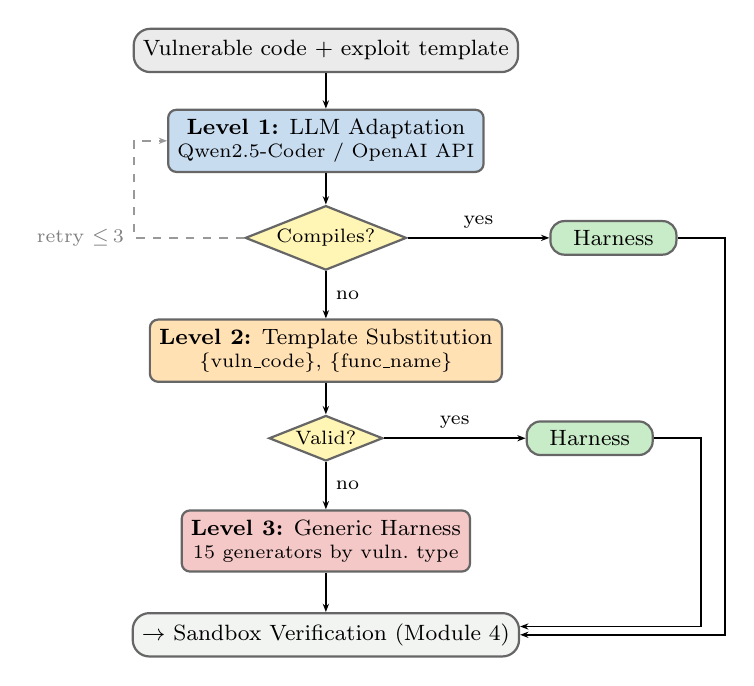
\begin{tikzpicture}[
    block/.style={rectangle, draw=black!60, rounded corners=3pt, minimum width=3.4cm,
        minimum height=0.55cm, align=center, font=\footnotesize, line width=0.8pt},
    decision/.style={diamond, draw=black!60, aspect=2.5, inner sep=1pt,
        font=\footnotesize, fill=decyellow, line width=0.8pt},
    success/.style={rectangle, draw=black!60, rounded corners=5pt, fill=modgreen,
        minimum width=1.6cm, minimum height=0.4cm, align=center, font=\footnotesize, line width=0.8pt},
    arr/.style={-{Stealth[length=3pt]}, semithick},
    darr/.style={-{Stealth[length=3pt]}, semithick, dashed, draw=black!40},
    node distance=0.35cm
]
\node[block, fill=modgray, rounded corners=6pt] (start) {Vulnerable code + exploit template};

\node[block, fill=modblue, below=0.45cm of start] (l1) {\textbf{Level 1:} LLM Adaptation\\[-1pt]{\scriptsize Qwen2.5-Coder / OpenAI API}};
\draw[arr] (start) -- (l1);

\node[decision, below=0.4cm of l1] (d1) {\scriptsize Compiles?};
\draw[arr] (l1) -- (d1);

\node[success, right=1.8cm of d1] (ok1) {Harness};
\draw[arr] (d1) -- node[above, font=\scriptsize] {yes} (ok1);

\draw[darr] (d1.west) -- ++(-1.4,0) node[left, font=\scriptsize, text=black!50]
    {retry ${\leq}\,3$} |- (l1.west);

\node[block, fill=modorange, below=0.6cm of d1] (l2) {\textbf{Level 2:} Template Substitution\\[-1pt]{\scriptsize \{vuln\_code\}, \{func\_name\}}};
\draw[arr] (d1) -- node[right, font=\scriptsize] {no} (l2);

\node[decision, below=0.4cm of l2] (d2) {\scriptsize Valid?};
\draw[arr] (l2) -- (d2);

\node[success, right=1.8cm of d2] (ok2) {Harness};
\draw[arr] (d2) -- node[above, font=\scriptsize] {yes} (ok2);

\node[block, fill=modred, below=0.6cm of d2] (l3) {\textbf{Level 3:} Generic Harness\\[-1pt]{\scriptsize 15 generators by vuln.\ type}};
\draw[arr] (d2) -- node[right, font=\scriptsize] {no} (l3);

\node[block, fill=modgreen!60!black!10, below=0.5cm of l3, rounded corners=6pt]
    (out) {$\to$ Sandbox Verification (Module 4)};
\draw[arr] (l3) -- (out);
\coordinate (routeR) at ([xshift=0.6cm]ok1.east);
\draw[arr] (ok1.east) -- (routeR) |- (out.east);
\draw[arr] (ok2.east) -- ([xshift=0.6cm]ok2.east) |- ([yshift=3pt]out.east);
\end{tikzpicture}%
}
\caption{Exploit template adaptation cascade. Upon failure at each level, control passes to the next: LLM adaptation with iterative refinement $\to$ template-based substitution $\to$ generic harness}
\label{fig:adaptation}
\end{figure}

\textit{Level~1: LLM adaptation} with iterative refinement~\cite{gajjar2026vbf}. An LLM (Qwen2.5-Coder-7B or OpenAI-compatible API) receives a structured prompt containing the vulnerable code, vulnerability type, the retrieved exploit template, and taint context (source$\to$sink paths), if available. Specialized hints are defined for 14~vulnerability types, directing the model toward generating specific exploit mechanisms. If the generated harness fails to compile, the system includes the compiler error message in the next prompt and retries the request (up to~3~attempts), allowing the LLM to correct the code.

\textit{Level~2: Template-based substitution.} If LLM adaptation fails (all attempts end in error or the LLM is unavailable), mechanical variable substitution is performed in the retrieved exploit template: vulnerable code, function name, and arguments.

\textit{Level~3: Generic harness.} If both previous levels fail, one of 15~specialized harness generators (one per supported vulnerability type) is guaranteed to return a minimal valid harness code that invokes the target function with potentially dangerous arguments.

The \texttt{adapt\_multi()} method generates multiple harness variants with MD5-hash-based deduplication, increasing the probability of successful verification.

\textbf{Sandbox verification.} Each generated harness is compiled and executed in a Docker-isolated environment with strict security constraints: \texttt{network=none}, \texttt{cap-drop=ALL}, a seccomp whitelist of 70+ allowed system calls, a memory limit of 1~GB, and PID~limit~128. This configuration prevents malicious code from escaping the container.

The system supports three mutually exclusive sanitizer profiles (Table~\ref{tab:sanitizers}) with automatic selection based on the vulnerability type. The \texttt{asan\_ubsan} profile (ASan~+ UBSan) detects buffer overflow, use-after-free, null~pointer dereference, and other memory errors. The \texttt{msan} profile (MemorySanitizer) specializes in detecting reads of uninitialized memory (CWE-457). The \texttt{tsan} profile (ThreadSanitizer) detects data races (CWE-362) and deadlocks (CWE-833). The mutual exclusivity is due to sanitizer incompatibility at the compiler instrumentation level.

\begin{table}
\centering
\caption{Sanitizer profiles for sandbox verification}
\label{tab:sanitizers}
\small
\begin{tabular}{|l|p{3.2cm}|p{4.0cm}|}
\hline
\textbf{Profile} & \textbf{Flags} & \textbf{Detects} \\
\hline
asan\_ubsan & \texttt{-fsanitize= address, undefined} & buffer overflow, UAF, null deref, int overflow \\
msan & \texttt{-fsanitize= memory} & uninit. read (CWE-457) \\
tsan & \texttt{-fsanitize= thread} & data race (CWE-362), deadlock (CWE-833) \\
\hline
\end{tabular}
\end{table}

Verification is two-phase. In the first phase, the harness is executed with predefined input data (static payload) with a 1-second timeout. If the sanitizer does not detect an error, the second phase is launched---coverage-guided fuzzing via LibFuzzer. To this end, an automatic transformation of \texttt{main()} $\to$ \texttt{LLVMFuzzerTestOneInput()} is performed: the system analyzes the \texttt{main()} signature and generates a wrapper that passes fuzzed data as arguments to the target function. LibFuzzer uses code coverage information to guide mutations, increasing the probability of detecting a vulnerability compared to random testing.

\textbf{Evidence classification and CWE mapping.} Sanitizer output is classified through 71~regular expression patterns (ASan:~17, UBSan:~14, MSan:~5, TSan:~7, Crash:~16, Valgrind:~12) into a four-level scale with confidence scoring (Table~\ref{tab:confidence}). Each pattern is assigned a base confidence level reflecting detection reliability: AddressSanitizer and MemorySanitizer produce the most reliable results (0.93--0.95), while indirect indicators (non-zero exit code) have significantly lower confidence (0.30).

Automatic CWE mapping (23~entries) matches each detected sanitizer pattern to a CWE identifier. For example, the \texttt{heap-buffer-overflow} pattern maps to CWE-122, \texttt{use-after-poison} maps to CWE-416, and \texttt{data race} maps to CWE-362.

The final verdict for each function under test is determined hierarchically: \textbf{CONFIRMED}---at least one harness is confirmed by a sanitizer or crash signal; \textbf{SUGGESTIVE}---indirect indicators are detected (Valgrind leak, non-zero exit); \textbf{NEUTRAL}---sandbox verification produced no results; \textbf{SAFE}---$S_{\text{hybrid}} < \tau$ (the function was not flagged as suspicious).

\begin{table}
\centering
\caption{Confidence scoring by evidence source}
\label{tab:confidence}
\small
\begin{tabular}{|l|c|c|}
\hline
\textbf{Source} & \textbf{Base confidence} & \textbf{Level} \\
\hline
ASan (17 patterns) & 0.95 & CONFIRMED \\
MSan (5 patterns) & 0.93 & CONFIRMED \\
TSan (7 patterns) & 0.91 & CONFIRMED \\
UBSan (14 patterns) & 0.90 & CONFIRMED \\
Crash/Signal (16 patterns) & 0.85 & CONFIRMED \\
Valgrind leak & 0.60 & SUGGESTIVE \\
Non-zero exit & 0.30 & SUGGESTIVE \\
Clean exit & 1.00 & SAFE \\
\hline
\end{tabular}
\end{table}

\textbf{LLM triage: parallel verification head.}
In parallel with sandbox verification, a second triage head based on an LLM (Claude Sonnet 4.6) operates as an independent validation channel. For each suspicious fragment, the system extracts a dependency graph via CodeQL, constructs a structured prompt containing the source code, graph context (data flows, function calls), and the suspected vulnerability type, and queries the LLM for classification (vulnerable~/~safe~/~uncertain).

The system implements asymmetric dual-head verification: the sandbox head provides execution-based evidence through sanitizers and fuzzing, while the LLM head provides semantic analysis with graph context. Cross-confirmation (both heads classify the function as vulnerable) significantly increases the confidence of the final verdict. Divergence in results (one head considers the code vulnerable, the other considers it safe) signals the need for manual review. The LLM head is particularly useful in cases where sandbox verification is difficult---for example, when a harness cannot be built due to complex dependencies---providing a fallback triage channel.


% ====================================================================
%              4. IMPLEMENTATION AND TESTING
% ====================================================================
\section{Implementation and Testing}

The system is implemented as a modular Python codebase\footnote{Source code: \url{https://github.com/deccersw/GNN-ReGVD-Plus}} comprising ${\sim}9,372$ lines with lazy initialization of modules (Table~\ref{tab:codebase}). The architecture follows the principle of separation of concerns: each pipeline module is encapsulated in a separate package with a well-defined interface. Lazy initialization ensures that heavy components (GNN model, FAISS indices, Docker client) are loaded only upon first access, which accelerates startup and reduces memory consumption when operating in sandbox-only mode.

\begin{table}
\centering
\caption{Codebase structure of GNN-ReGVD+}
\label{tab:codebase}
\small
\begin{tabular}{|l|l|r|}
\hline
\textbf{Module} & \textbf{Main components} & \textbf{Lines} \\
\hline
\texttt{code/} & GNN model, FAISS index, inference engine & ${\sim}2,800$ \\
\texttt{exploit\_db/} & Exploit index, adapter, templates & ${\sim}1,500$ \\
\texttt{sandbox/} & Executor, evidence classifier, Docker & ${\sim}1,500$ \\
\texttt{analysis/} & Taint analysis (Joern CPG / regex) & ${\sim}400$ \\
\texttt{scanner/} & Pipeline orchestrator, config, report & ${\sim}600$ \\
\texttt{tests/} & 203 automated tests & ${\sim}2,500$ \\
CLI + evaluate & \texttt{scan\_cli.py}, \texttt{evaluate.py} & ${\sim}570$ \\
\hline
\textbf{Total} & & ${\sim}$\textbf{9,372} \\
\hline
\end{tabular}
\end{table}

The CLI interface (\texttt{scan\_cli.py}) supports three operating modes: single function analysis (interactive input or file), batch scanning of JSONL datasets, and sandbox-only mode (verification without GNN detection). The system automatically detects GPU availability and switches between CUDA and CPU inference. Pipeline configuration (thresholds, hyperparameters, model paths) is managed through a single YAML file with schema validation.

\textbf{Testing.} 203~automated tests cover all system modules: sandbox (61~tests), enhancements (55), exploit adapter (36), pipeline (25), evaluation (18), and FAISS (11). Tests are designed to run without GPU, Docker, or a trained model---all external dependencies are mocked. The execution time for the full test suite is ${\sim}6$~seconds. Testing includes unit tests for individual components (sanitizer output parsing, CWE mapping, harness generation), integration tests (function traversal through the complete pipeline with mocked external services), and regression tests for detection result reproducibility.


% ====================================================================
%              5. EXPERIMENTAL EVALUATION
% ====================================================================
\section{Experimental Evaluation}

\subsection{Experimental Protocol and Data}

The experimental program comprises four sequential phases aimed at evaluating each component of the hybrid architecture:

\begin{itemize}
    \item \textbf{Phase~1:} Reproduction of the ReGVD baseline on the Devign dataset to confirm implementation correctness.
    \item \textbf{Phase~2:} Training of the hybrid model (ReGVD + LoRA + FAISS) on Devign to evaluate component compatibility.
    \item \textbf{Phase~3:} Zero-shot transfer of the Devign-trained model to the MegaVul dataset for quantitative assessment of the domain gap.
    \item \textbf{Phase~4:} LoRA adaptation on MegaVul to evaluate the effectiveness of parameter-efficient domain transfer.
\end{itemize}

Two datasets were used:
\begin{itemize}
    \item \textbf{Devign}~\cite{zhou2019devign}: 27,318 C functions from four major open-source projects (QEMU, FFmpeg, Linux Kernel, Wireshark). The class distribution is approximately balanced (${\sim}45.6$\% vulnerable functions), which simplifies training but does not reflect the real distribution of vulnerabilities in production code.
    \item \textbf{MegaVul}~\cite{ni2024megavul}: 339,548 C/C++ functions from 992~open-source projects. Contains ${\sim}5.1$\% vulnerable functions (169~CWE types), which is significantly closer to the real-world distribution. The scale and diversity make MegaVul a considerably more challenging benchmark.
\end{itemize}

\textbf{Hardware environment}: 1$\times$ NVIDIA RTX 3090 (24~GB VRAM), AMD Ryzen~9, 64~GB RAM, Ubuntu~22.04.

\textbf{Model hyperparameters}: block\_size~=~400 (maximum token sequence length), window\_size~=~5 (sliding window size for graph construction), ReGCN ($L{=}2$ layers, $h{=}128$ hidden units), batch\_size~=~128, AdamW optimizer ($\text{lr} = 5 \times 10^{-4}$, weight decay $= 10^{-2}$), contrastive loss weight $\alpha = 0.7$, SupCon temperature $\tau = 0.07$.

\textbf{LoRA hyperparameters}: $r = 8$, $\alpha = 16$, $\text{lr} = 1 \times 10^{-4}$, replay\_ratio~=~0.2 (fraction of examples from the original domain in each batch to prevent catastrophic forgetting).


\subsection{Results and Analysis}

\textbf{Phases~1--2: Devign.}
Reproduction of the ReGVD baseline confirmed implementation correctness (Accuracy~=~0.646, F1~=~0.571, ROC-AUC~=~0.704). The introduction of LoRA adapters, the embedding head, and the FAISS index did not lead to a significant change in quality: the deviation across all metrics was less than 0.5~p.p. (Table~\ref{tab:summary}, columns Ph.~1 and Ph.~2). This result confirms the compatibility of the added components with the base architecture: the contrastive component $\mathcal{L}_{\text{SupCon}}$ forms an embedding space orthogonal to the binary classification task, introducing no destructive interference. The slight increase in trainable parameters (from ${\sim}12.7$M to ${\sim}13.0$M) does not lead to overfitting due to the regularizing effect of LoRA.

\textbf{Phases~3--4: MegaVul (domain transfer).}
Zero-shot transfer of the model trained on the balanced Devign to the imbalanced MegaVul showed a substantial drop in metrics (ROC-AUC: $0.700 \to 0.572$, F1: $0.575 \to 0.124$), confirming a significant domain gap between the datasets (Table~\ref{tab:summary}, columns Ph.~3 and Ph.~4). The main causes of the drop: (1)~class distribution difference (45.6\% vs. 5.1\% vulnerable), (2)~code style difference (4~projects vs. 992~projects), (3)~vulnerability type difference (Devign lacks CWE annotations, MegaVul has 169~CWE types).

LoRA adaptation with training of only 0.12\% of parameters (${\sim}152.8$K out of ${\sim}125$M) substantially recovered quality: ROC-AUC~$+0.179$, Precision increased 5$\times$ (from 0.073 to 0.367), F1 increased 2.3$\times$ (from 0.124 to 0.284). Accuracy grew from 0.621 to 0.928, which is explained by correct model calibration on the imbalanced distribution: the model learned to predict the negative class for the majority of functions, consistent with the actual class ratio.

The decrease in Recall ($0.428 \to 0.231$) is an expected result of calibration: with ${\sim}5.1$\% vulnerable functions, high Recall inevitably accompanies low Precision. The chosen trade-off (Precision~=~0.367, Recall~=~0.231) corresponds to the practical task where the cost of a false positive (unnecessary sandbox verification) is substantially lower than the cost of a missed vulnerability, but an excessively high false positive rate makes the system impractical.

\textbf{Summary results.}
Table~\ref{tab:summary} summarizes the results of all four experimental phases. Key observations: (1)~the hybrid architecture is neutral to the baseline quality on the original domain; (2)~the domain gap between balanced and imbalanced datasets is significant; (3)~LoRA adaptation effectively overcomes the domain gap with minimal computational cost.

\begin{table}
\centering
\caption{Summary results of the experimental phases}
\label{tab:summary}
\small
\begin{tabular}{|l|*{4}{c|}}
\hline
\textbf{Metric} & \textbf{Ph.~1: ReGVD} & \textbf{Ph.~2: Hybrid} & \textbf{Ph.~3: Zero-shot} & \textbf{Ph.~4: + LoRA} \\
& \footnotesize (Devign) & \footnotesize (Devign) & \footnotesize (MegaVul) & \footnotesize (MegaVul) \\
\hline
Accuracy & 0.646 & 0.645 & 0.621 & \textbf{0.928} \\
ROC-AUC & 0.704 & 0.700 & 0.572 & \textbf{0.751} \\
F1 & 0.571 & 0.575 & 0.124 & \textbf{0.284} \\
Precision & 0.603 & 0.599 & 0.073 & \textbf{0.367} \\
Recall & 0.543 & 0.552 & 0.428 & 0.231 \\
Train. params & ${\sim}12.7$M & ${\sim}13.0$M & --- & ${\sim}$\textbf{152.8K} \\
\hline
\end{tabular}
\end{table}

\textbf{System performance.}
Table~\ref{tab:performance} presents system performance characteristics. The inference latency increase is ${\sim}21$\% (from 28~ms to 34~ms) due to the embedding head and FAISS search. This increase is acceptable for CI/CD integration: at a throughput of ${\sim}29$~functions/s, a full scan of a project with 10,000~functions takes less than 6~minutes. Inference VRAM increased slightly (from 1.9~GB to 2.1~GB), allowing inference even on budget GPUs.

The main resource benefit is achieved during fine-tuning: VRAM decreases from ${\sim}14.2$~GB to ${\sim}7.8$~GB (1.8$\times$), and energy consumption from ${\sim}1.92$~kWh to ${\sim}0.23$~kWh (${\sim}8\times$). In terms of CO$_2$ equivalent, this represents a reduction from ${\sim}920$~g to ${\sim}110$~g per fine-tuning cycle.

\begin{table}
\centering
\caption{System performance (NVIDIA RTX 3090)}
\label{tab:performance}
\small
\begin{tabular}{|l|c|c|}
\hline
\textbf{Metric} & \textbf{ReGVD baseline} & \textbf{Hybrid} \\
\hline
Inference latency, ms & ${\sim}28$ & ${\sim}34$ \\
Throughput, functions/s & ${\sim}36$ & ${\sim}29$ \\
VRAM at inference, GB & ${\sim}1.9$ & ${\sim}2.1$ \\
VRAM at fine-tuning, GB & ${\sim}14.2$ & ${\sim}$\textbf{7.8} \\
Hot-update (100 emb.), s & --- & ${\sim}0.18$ \\
Fine-tuning energy, kWh & ${\sim}1.92$ & ${\sim}$\textbf{0.23} \\
CO$_2$ equivalent, g & ${\sim}920$ & ${\sim}$\textbf{110} \\
\hline
\end{tabular}
\end{table}

\textbf{Vulnerability type coverage.}
Table~\ref{tab:vuln_coverage} presents the coverage matrix: the sandbox verification module supports 18~vulnerability types (23~CWE entries). For each type, the availability of exploit templates, generic generators, the sanitizer profile used, and taint analysis support are indicated. Memory-related vulnerabilities (buffer overflow, UAF, format string) have the most comprehensive coverage: specialized templates, generic generators, taint analysis, and the ASan sanitizer are all available. Concurrency vulnerabilities (data race, deadlock) are covered through TSan but without taint analysis, as taint analysis is oriented toward data flows rather than inter-thread interactions.

\begin{table}
\centering
\caption{Vulnerability type coverage matrix}
\label{tab:vuln_coverage}
\small
\begin{tabular}{|l|l|c|c|c|c|}
\hline
\textbf{Vulnerability type} & \textbf{CWE} & \textbf{Templ.} & \textbf{Generic} & \textbf{Sanit.} & \textbf{Taint} \\
\hline
Buffer Overflow (stack) & CWE-121 & 3 & \checkmark & ASan & \checkmark \\
Buffer Overflow (heap) & CWE-122 & 2 & \checkmark & ASan & \checkmark \\
Use-After-Free & CWE-416 & 2 & \checkmark & ASan & \checkmark \\
Double-Free & CWE-415 & --- & \checkmark & ASan & \checkmark \\
Format String & CWE-134 & 2 & \checkmark & ASan & \checkmark \\
Integer Overflow & CWE-190 & 2 & \checkmark & UBSan & --- \\
Null Pointer Deref & CWE-476 & 2 & \checkmark & ASan & --- \\
Off-by-One & CWE-193 & 2 & \checkmark & ASan & \checkmark \\
Division by Zero & CWE-369 & 2 & \checkmark & UBSan & --- \\
Uninit. Read & CWE-457 & 2 & \checkmark & MSan & --- \\
Data Race & CWE-362 & 1 & \checkmark & TSan & --- \\
Deadlock & CWE-833 & --- & --- & TSan & --- \\
\hline
\end{tabular}
\end{table}

\textbf{LLM triage results.}
The LLM triage head (Claude Sonnet 4.6 + CodeQL) was evaluated on a held-out sample of 848~examples (Table~\ref{tab:llm_triage}). Accuracy was 69.6\%, with recall on the vulnerable class of 81.6\% (346 out of 424), which corresponds to a conservative calibration: the cost of missing a real vulnerability (false negative) is substantially higher than the cost of a false positive. Recall on the safe class was 57.1\% (242 out of 424), indicating a tendency of the LLM toward over-reporting vulnerabilities.

The proportion of uncertain responses was only 0.35\% (3~out of~848), confirming the stability of the response format and the suitability of the LLM head for automated integration without manual post-processing. The cost per query is ${\sim}\$0.006$, making LLM triage economically feasible even at scale.

\begin{table}
\centering
\caption{LLM triage head results ($N = 848$)}
\label{tab:llm_triage}
\small
\begin{tabular}{|l|c|c|}
\hline
\textbf{Metric} & \textbf{Value} & \textbf{Comment} \\
\hline
Accuracy & 69.6\% & excluding uncertain \\
True positives & 346/424 & Recall: 81.6\% \\
True negatives & 242/424 & Recall: 57.1\% \\
Uncertain & 3 & 0.35\% \\
Cost per query & \$0.006 & Claude Sonnet 4.6 \\
\hline
\end{tabular}
\end{table}


% ====================================================================
%              6. CONCLUSION
% ====================================================================
\section{Conclusion}

This work proposes an integrated vulnerability scanner architecture, GNN-ReGVD+, combining four modules: GNN detection based on the ReGVD model with LoRA adaptation and hybrid scoring via FAISS, exploit template retrieval from a vector database, cascading LLM template adaptation with iterative refinement, and multi-sanitizer sandbox verification (ASan+UBSan, MSan, TSan) with coverage-guided fuzzing via LibFuzzer. An LLM triage head based on Claude Sonnet 4.6 with CodeQL graph context operates in parallel.

Experimental evaluation on the Devign (27,318~functions) and MegaVul (339,548~functions) datasets confirmed four key results: (a)~the hybrid architecture does not degrade baseline model performance on the original domain ($\Delta < 0.5$~p.p. across all metrics); (b)~LoRA adaptation of 0.12\% of parameters (${\sim}152.8$K out of ${\sim}125$M) yields a ROC-AUC improvement of $+0.179$ during domain transfer with a 1.8$\times$ VRAM reduction and 8$\times$ energy savings; (c)~multi-sanitizer verification covers 18~vulnerability types (23~CWE entries) with four-level evidence classification; (d)~the LLM triage head achieves 81.6\% recall on the vulnerable class at a cost of \$0.006 per query. The implementation (9,372~lines of Python code, 203~automated tests, CLI interface) is oriented toward CI/CD integration.

The system's limitations include: support for C/C++ only, modest Recall on imbalanced data (0.231 on MegaVul), Docker overhead (${\sim}2$--5~s per harness), LLM triage accuracy of 69.6\%, and a limited database of 20~exploit templates. Promising directions for future development include extending language support (Python, Java), applying class imbalance strategies (focal loss, class-balanced sampling), reducing sandbox overhead via container pools, integrating symbolic execution (KLEE), and expanding the template database from CVEfixes and DiverseVul.


%
\begin{credits}
\subsubsection{\discintname}
The authors declare no conflict of interest.
\end{credits}
%
% ---- Bibliography ----
%
\begin{thebibliography}{17}

\bibitem{nguyen2022regvd}
Nguyen~V.-A., Nguyen~D.\,Q., Nguyen~V., Le~T., Tran~Q.\,H., Phung~D.:
ReGVD: Revisiting Graph Neural Networks for Vulnerability Detection.
In: Proc. ICSE '22 Companion, pp.~164--165 (2022)

\bibitem{zhou2019devign}
Zhou~Y., Liu~S., Siow~J., Du~X., Liu~Y.:
Devign: Effective Vulnerability Identification by Learning Comprehensive Program Semantics via Graph Neural Networks.
arXiv preprint arXiv:1909.03496 (2019)

\bibitem{guo2021graphcodebert}
Guo~D., Ren~S., Lu~S. et~al.:
GraphCodeBERT: Pre-training Code Representations with Data Flow.
arXiv preprint arXiv:2009.08366 (2021)

\bibitem{hu2021lora}
Hu~E.\,J., Shen~Y., Wallis~P. et~al.:
LoRA: Low-Rank Adaptation of Large Language Models.
arXiv preprint arXiv:2106.09685 (2021)

\bibitem{khosla2020supcon}
Khosla~P. et~al.:
Supervised Contrastive Learning.
In: NeurIPS, vol.~33, pp.~18661--18673 (2020)

\bibitem{johnson2019faiss}
Johnson~J., Douze~M., J\'{e}gou~H.:
Billion-scale Similarity Search with GPUs.
IEEE Trans. Big Data \textbf{7}(3), 535--547 (2019)

\bibitem{ding2024}
Ding~Y., Fu~Y., Ibrahim~O. et~al.:
Vulnerability Detection with Code Language Models: How Far Are We?
arXiv preprint arXiv:2403.18624 (2024)

\bibitem{sultana2024}
Sultana~Sh., Afrin~S., Eisti~N.\,Y.:
Code Vulnerability Detection: A Comparative Analysis of Emerging Large Language Models.
arXiv preprint arXiv:2409.10490 (2024)

\bibitem{makhyari2024}
Makhyari~A.\,A.:
Harnessing the Power of LLMs in Source Code Vulnerability Detection.
arXiv preprint arXiv:2408.03489 (2024)

\bibitem{li2025neurosymbolic}
Li~P. et~al.:
Neuro-symbolic Static Analysis with LLM-generated Vulnerability Patterns.
arXiv preprint arXiv:2504.16057 (2025)

\bibitem{gajjar2026vbf}
Gajjar~M.:
Verify Before You Fix: Execution-Based Validation for LLM-Generated Vulnerability Patches.
arXiv preprint (2026)

\bibitem{agrawal2025sast}
Agrawal~A., Ahi~P.:
SAST-Genius: LLM-Based Triage and PoC Generation for SAST Alerts.
arXiv preprint (2025)

\bibitem{ni2024megavul}
Ni~C., Shen~L., Yang~X., Zhu~Y., Wang~S.:
MegaVul: A C/C++ Vulnerability Dataset with Comprehensive Code Representations.
In: Proc. MSR~'24, pp.~738--742 (2024)

\bibitem{chen2024uaf}
Chen~X., Li~Y., Wang~Z.:
Use-After-Free Vulnerability Detection via Deep Graph Learning.
IEEE Trans. Software Engineering \textbf{50}(4), 1123--1139 (2024)

\bibitem{nist800}
NIST:
Risk Management Guide for Information Technology Systems.
NIST SP 800-30 Rev.~1 (2023)

\bibitem{owasp2024}
OWASP Foundation:
OWASP Top 10:2024~--- The Ten Most Critical Web Application Security Risks (2024)

\bibitem{seacord2021}
Seacord~R.\,C.:
Secure Coding in C and C++, 3rd edn. Addison-Wesley, Boston (2021)

\end{thebibliography}

\end{document}
